\chapter{Using the Hadoop Streaming Interface with Python}

\begin{fullwidth}
{\em in progress}

\section{Goal}

Your goal in this lab is to learn how to launch a simple map-reduce job at Amazon using their elastic map reduce mechanism. Our application is the trite ``word counting.'' You'll use Python as in the other labs.

\section{Discussion}

Hadoop is written in Java and so to use another language, such as Python, we have to use the so-called {\em streaming interface}. That just means that we will write programs that read from standard input and write to standard output. Hadoop is a distributed computing framework that supports a \href{http://wiki.apache.org/hadoop/HadoopMapReduce}{\textcolor{blue}{map-reduce computing paradigm}}. The {\em map} operation executes on multiple machines and gets partial results, which are then combined with the {\em reduce} operation. Hadoop splits the input into chunks and gives each  chunk to a mapper, which generates partial results. These partial results are a set of key-value pairs. Hadoop  sorts these according to key and distributes regions of the key space across one or more reducers. The reducer is responsible for generating the final result. 

We will be using Amazon Elastic MapReduce (EMR) that will take care of all the details of launching a cluster, running our job, and creating the output files. In Amazons par loss, we will be adding a {\em step} that represents our map-reduce job.

The hadoop file system (HDFS) is a distributed file system that can handle massive amounts of data by distributing it across multiple machines and hard drives. Hadoop tries to keep map operations on the machines that store the associated data the mappers should run on. That is what typically is done, but we will be using Amazons S3 storage instead since it is the easiest thing to do.

A hadoop {\em job} is a chunk of work, which can have one or more tasks. If one of these tasks fails, hadoop tries to rerun them. AWS introduces the notion of a {\em step}, which is one of more jobs. We will be using one step that consists of a mapper and reducer written in Python.

Hadoop streaming likes to generate an output file per reducer, which can be handy if we are interested in partitioning, say, sales results per country. In that case, we would have one reducer per country.  When I asked for three reducers, I got the following files in my output folder:

\scalebox{.65}{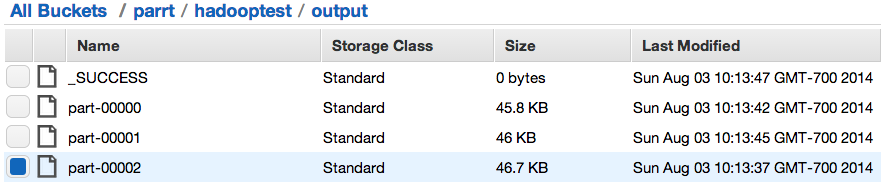
\includegraphics{figures/3reducers-output.png}}


\begin{alltt}\small
python wcmap.py < ~/courses/CS680/data/ads1000.txt |sort| python wcreduce.py | sort > output.txt
\end{alltt}

\section{Resources}

You will find {\tt wcmap.py} and {\tt wcreduce.py} at github.

\section{Deliverables}

None. Please follow along in class.

\end{fullwidth}
